% The two chains and the interleaver of Section~\ref{sec:turbo}, drawn by
% hand. Input by textbook.tex; a sketch and not a rendered figure, so it is
% outside the figure cache and the render cap, which govern generated output
% only.
\begin{figure}[htbp]
\centering
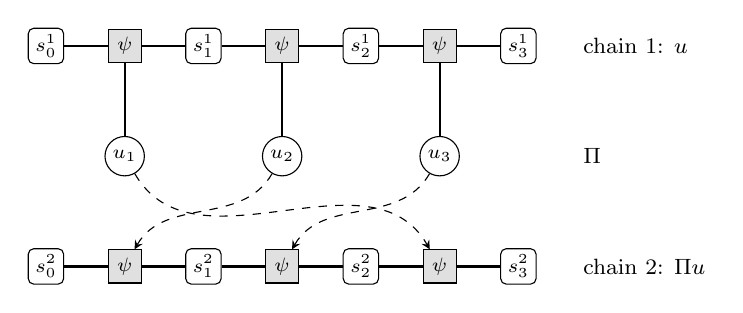
\begin{tikzpicture}[
    scale=1.0,
    bit/.style={circle, draw, minimum size=0.5cm, inner sep=0.5pt, font=\scriptsize, fill=white},
    state/.style={rectangle, draw, rounded corners=2pt, minimum size=0.45cm, inner sep=1pt, font=\scriptsize, fill=white},
    trell/.style={rectangle, draw, fill=black!12, minimum size=0.42cm, inner sep=1pt, font=\scriptsize},
    link/.style={draw, thick},
    perm/.style={draw, dashed, ->, >=stealth}
]
  % first chain
  \foreach \i/\x in {0/1.6, 1/3.6, 2/5.6, 3/7.6} {
    \node[state] (s\i) at (\x, 3.0) {$s^{1}_{\i}$};
  }
  \foreach \i/\j/\x in {0/1/2.6, 1/2/4.6, 2/3/6.6} {
    \node[trell] (t\i) at (\x, 3.0) {$\psi$};
    \draw[link] (s\i) -- (t\i); \draw[link] (t\i) -- (s\j);
  }
  \node[anchor=west, font=\footnotesize] at (8.3, 3.0) {chain 1: $u$};
  % message bits
  \foreach \i/\x in {1/2.6, 2/4.6, 3/6.6} {
    \node[bit] (u\i) at (\x, 1.6) {$u_{\i}$};
  }
  \draw[link] (t0) -- (u1);
  \draw[link] (t1) -- (u2);
  \draw[link] (t2) -- (u3);
  % second chain
  \foreach \i/\x in {0/1.6, 1/3.6, 2/5.6, 3/7.6} {
    \node[state] (r\i) at (\x, 0.2) {$s^{2}_{\i}$};
  }
  \foreach \i/\j/\x in {0/1/2.6, 1/2/4.6, 2/3/6.6} {
    \node[trell] (v\i) at (\x, 0.2) {$\psi$};
    \draw[link] (r\i) -- (v\i); \draw[link] (v\i) -- (r\j);
  }
  \node[anchor=west, font=\footnotesize] at (8.3, 0.2) {chain 2: $\Pi u$};
  \draw[perm] (u1) to[out=-60, in=120] (v2);
  \draw[perm] (u2) to[out=-120, in=60] (v0);
  \draw[perm] (u3) to[out=-120, in=60] (v1);
  \node[anchor=west, font=\footnotesize] at (8.3, 1.6) {$\Pi$};
\end{tikzpicture}
\caption{A turbo code as a factor graph: two trellis chains sharing the
message bits through a permutation. Each $\psi$ is one trellis factor of
Equation~\ref{eq:turbo-factor}, carrying both the transition the register
allows and the channel's score for the two bits that transition transmits;
each $s^{c}_{t}$ is a register state. The message bit $u_i$ is read by the
first chain at position $i$ and by the second at position $\Pi^{-1}(i)$, so
every $u_i$ has degree two and the graph has one cycle per pair of message
bits the permutation reorders --- which is why
Equation~\ref{eq:sum-product} on it is the Bethe approximation and why the
serial schedule of Algorithm~\ref{alg:turbo-decode} is a choice rather than
a derivation. Three message bits and a memory-1 register are drawn; the
instances this repository carries are $K = 12$, $256$ and $1{,}024$ with the
memory-2 $(7,5)$ register. A sketch of the structure and not a rendering of
any instance.}
\label{fig:turbo:sketch}
\end{figure}
